
\newcommand{\depBox}[1]{
	\begin{adjustbox}{minipage=0.85\textwidth,margin=0 \smallskipamount,center}
		Abhängigkeiten:	 \quad #1
	\end{adjustbox} ~\\
}
\newcommand{\refModCore}{\hyperref[mod_core]{Core}}
\newcommand{\refModData}{\hyperref[mod_data]{Data}}
\newcommand{\refModDataUI}{\hyperref[mod_data-ui]{Data-UI}}
\newcommand{\refModJavaFX}{\hyperref[mod_javafx]{JavaFX}}
\newcommand{\refModModel}{\hyperref[mod_model]{Model}}
\newcommand{\refModStorage}{\hyperref[mod_storage]{Storage}}

\section{Module}
\subsection{Modulübersicht}
Die Teilbereiche des Projekts wurden in verschieden Module aufgeteilt:
\begin{figure}[hb!]
	\centering
	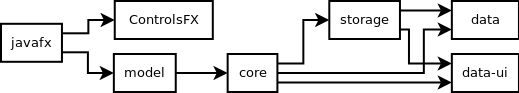
\includegraphics[width=.8\textwidth]{module_dependencies.png}
	\caption{Abhängigkeitsgraph der Module}
	\label{mod_dep_view}
\end{figure}

Der in Abbildung \ref{mod_dep_view} gezeigte Graph enthält keine Abhängigkeiten nach JUnit und
dem JDK aus Gründen der Übersicht.

Anzumerken ist auch, dass bis in das Modul \refModCore{} keine Abhängigkeiten
gegenüber einer UI-Bibliothek existieren. Das Modul \hyperref[mod_data-ui]{Data-UI} stellt
zwar Komponenten bereit, die für die Integration in eine Benutzeroberfläche benötigt werden,
bleibt jedoch Benutzeroberflächenunabhängig.

fasdf asdf asdf asd



\subsection{Modul Core}
\label{mod_core}
\depBox{Data (\ref{mod_data}), Data-UI (\ref{mod_data-ui}), Storage (\ref{mod_storage})}

Modulerklräung hier




\subsection{Modul Data}
\label{mod_data}
\depBox{Keine}

Modulerklräung hier




\subsection{Modul Data-UI}
\label{mod_data-ui}
\depBox{Keine}

Modulerklräung hier




\subsection{Modul JavaFX}
\label{mod_javafx}
\depBox{Model (\ref{mod_model}), ControlsFX (ext. \cite{controlsfx})}

Modulerklräung hier




\subsection{Modul Model}
\label{mod_model}
\depBox{Core (\ref{mod_core})}

Modulerklräung hier




\subsection{Modul Storage}
\label{mod_storage}
\depBox{Data (\ref{mod_data}), Data-UI (\ref{mod_data-ui})}

Modulerklräung hier

